

\newcommand{\DqBeschreibung}[3]{\textbf{Name der Datenquelle: }#1 \textbf{Format: }#3 \\ \textbf{Kurszbeschreibung:} #2 \\  \\}

\newcommand{\Quellattribut}[2]{ \textbf{Attributname}: #1 \textbf{Beschreibung}: #2 \\ }
\section{Datenquellen}
\newcommand{\SsisTask}[1]{\emph{#1} \index{SSIS Task!#1}}
\newcommand{\SsisPack}[1]{\emph{#1} \index{SSIS Package!#1}}

\subsection{DataProfilingTaskSample}
\DqBeschreibung{DataProfilingTaskSample}{Ein einfache Datenquelle, die zum Testen gebaut habe}{csv}
\Quellattribut{ID}{Fortlaufende ID}
\Quellattribut{Geschlecht} {In der Kodierung m und w}
\Quellattribut{Alter}{Alter als numerischer String. Werte sollen zwischen 0 und 130 liegen}
\Quellattribut{Verm�gen}{Numerischer Ganzzahl String}


\section{Datenintegration}
\subsection{DataProfilingTaskSample}
\subsection{Extraktion}
Hier steht der beschreibne Text, wie das realisiert \\
\textbf{Bsonderheiten: } Hier musste man eine Ausnahme von dem Vorgen in \ref{BP_Extract} gemacht, da hier die Daten anders sind.
\subsection{Kodierung}
\subsection{Struktur}
\subsection{Umsetzung Fachlichkeit} Hier muss die Regel \ref{BP_Extract} Anwendung finden, da ... Realisiert wurde dies mit der SIS Komponenten.


\section{Datenintegration: DataProfilingTaskSample}
Ein einfaches Beispiel f�r die Datenquellen
\subsection{Extraktion}
Hier wird mittels csv flatfile Import realisiert
\textbf{Bsonderheiten: } Hier musste man eine Ausnahme von dem Vorgen in \ref{BP_Extract} gemacht, da hier die Daten anders sind.
\subsection{Kodierung}
\subsection{Vollst�ndigkeit und Struktur}
Die Vollst�ndigkeit und die Struktur wird in dem Paket \SsisPack{Bereinigung.dtsx} realisiert. Und ist in der Abbildung  dargestellt. Zuerst wird auf leere oder null-Werte �berpr�ft und aussortiert. Dies passiert im Task \SsisTask{CheckNullOrEmptyColumns}. Haben Zeilen leere Werte, werden diese komplett aussortiert und in die Tabelle eingef�gt\\

Die L�nge der Datentypen und die Formatieren werden im Task \SsisTask{Length and type Check} ausgef�hrt. Hier wird die L�nge des Geschlecht und ob es sich bei Alter um eine Zahl handelt.

\paragraph{SISS Paket}
\begin{figure}
	\centering
		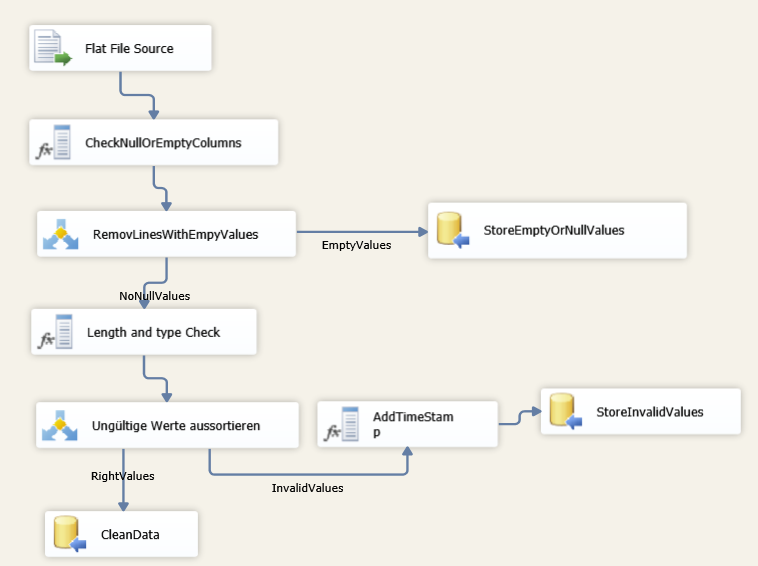
\includegraphics[width=1.00\textwidth]{doku/Bilder/DataProfilingTaskSampleVollstaendigkeitUndStrukturSISS.PNG}
	\caption{Vollst�ndigkeit und Struktur SISS Paket}
	\label{fig:DataProf}
\end{figure}
\paragraph{Verwendete Logging Tabellen}
\begin{figure}
	\centering
		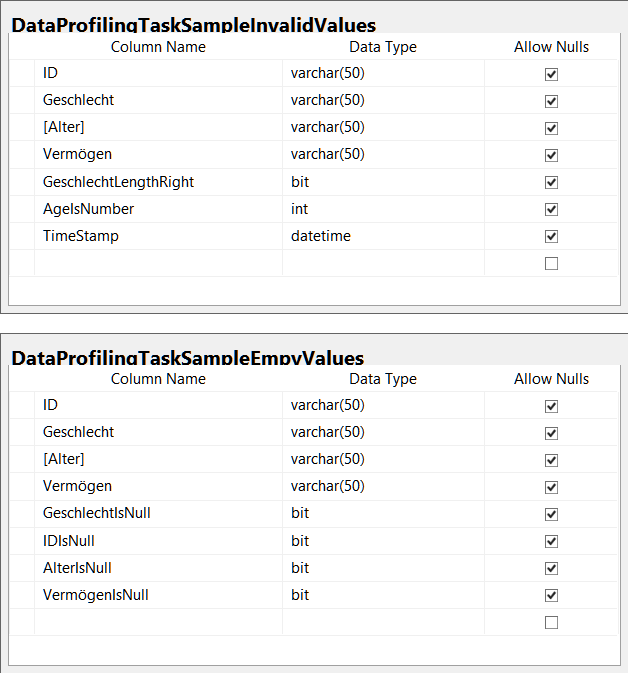
\includegraphics[width=0.70\textwidth]{doku/Bilder/LoggingTables.png}
	\caption{Logging Tabellen}
	\label{fig:LoggingTables}
\end{figure}



�berpr�ft werden m�ssen die Felder
\subsection{Umsetzung Fachlichkeit} Hier muss die Regel \ref{Rule:WertebereichAlter} Anwendung finden, da ... Realisiert wurde dies mit der SSIS Komponente \SsisTask{Fachliche Regel Alter}
\begin{lstlisting}
(DT_I4)Alter >= 0 && (DT_I4)Alter <= 130
\end{lstlisting}
\textbf{Realisiert in Package: } ExtractIncidentReport.dtsx
\section{Zentrale Datenhaltung}
\section{Aggregation}
\section{Reporting}
\section{Fachliche Reglen}
\subsection{Geschlecht zu ICD}\label{GeschlechtZuICD}
\subsection{Wertebereich Alter:}\label{Rule:WertebereichAlter}
Ein Alter darf nur zwischen 0 und 130 liegen

\textbf{Fachliche Beschreibung: }wenn ein ICD 40 oder 50 lautet dann kann das Geschlecht nur weiblich sein.\\
\textbf{Dom�nenexperte} Herr Sander \\
